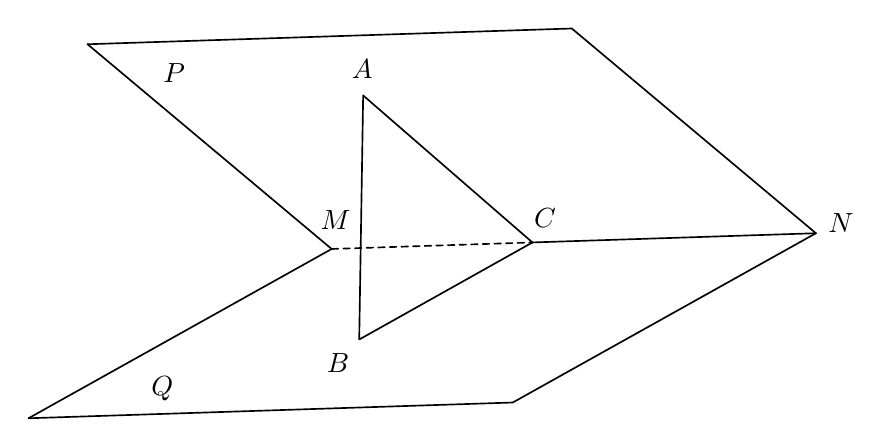
\begin{tikzpicture}[x=1cm,y=1cm,line width=.6pt,line cap=round,line join=round]
  \tikzset{
    gedge/.style={line width=.6pt},
    ghidden/.style={line width=.6pt,dash pattern=on 2.4pt off 1.8pt},
    glabel/.style={inner sep=1.5pt,font=\normalsize}
  }
  \coordinate (P1) at (1.85,5.65);
  \coordinate (P2) at (8.00,5.85);
  \coordinate (N) at (11.10,3.25);
  \coordinate (M) at (4.95,3.05);
  \coordinate (Q1) at (1.10,0.90);
  \coordinate (Q2) at (7.25,1.10);
  \coordinate (A) at (5.35,5.00);
  \coordinate (B) at (5.30,1.90);
  \coordinate (C) at (7.50,3.132927);
  \draw[gedge] (P1)--(P2)--(N);
  \draw[gedge] (M)--(P1);
  \draw[gedge] (Q1)--(Q2)--(N);
  \draw[gedge] (M)--(Q1);
  \draw[ghidden] (M)--(C);
  \draw[gedge] (C)--(N);
  \draw[gedge] (A)--(B)--(C)--cycle;
  \node[glabel] at (2.95,5.28) {$P$};
  \node[glabel] at (2.80,1.28) {$Q$};
  \node[glabel] at (5.00,3.42) {$M$};
  \node[glabel] at (11.42,3.38) {$N$};
  \node[glabel] at (5.34,5.34) {$A$};
  \node[glabel] at (5.03,1.60) {$B$};
  \node[glabel] at (7.66,3.44) {$C$};
\end{tikzpicture}
